%% abtex2-modelo-trabalho-academico.tex, v-1.9.7 laurocesar
%% Copyright 2012-2018 by abnTeX2 group at http://www.abntex.net.br/ 
%%
%% This work may be distributed and/or modified under the
%% conditions of the LaTeX Project Public License, either version 1.3
%% of this license or (at your option) any later version.
%% The latest version of this license is in
%%   http://www.latex-project.org/lppl.txt
%% and version 1.3 or later is part of all distributions of LaTeX
%% version 2005/12/01 or later.
%%
%% This work has the LPPL maintenance status `maintained'.
%% 
%% The Current Maintainer of this work is the abnTeX2 team, led
%% by Lauro César Araujo. Further information are available on 
%% http://www.abntex.net.br/
%%
%% This work consists of the files abntex2-modelo-trabalho-academico.tex,
%% abntex2-modelo-include-comandos and abntex2-modelo-references.bib
%%

% ------------------------------------------------------------------------
% ------------------------------------------------------------------------
% abnTeX2: Modelo de Trabalho Academico (tese de doutorado, dissertacao de
% mestrado e trabalhos monograficos em geral) em conformidade com 
% ABNT NBR 14724:2011: Informacao e documentacao - Trabalhos academicos -
% Apresentacao
% ------------------------------------------------------------------------
% ------------------------------------------------------------------------

\documentclass[
	% -- opções da classe memoir --
	12pt,				% tamanho da fonte
	openright,			% capítulos começam em pág ímpar (insere página vazia caso preciso)
	twoside,			% para impressão em recto e verso. Oposto a oneside
	a4paper,			% tamanho do papel. 
	% -- opções da classe abntex2 --
	%chapter=TITLE,		% títulos de capítulos convertidos em letras maiúsculas
	%section=TITLE,		% títulos de seções convertidos em letras maiúsculas
	%subsection=TITLE,	% títulos de subseções convertidos em letras maiúsculas
	%subsubsection=TITLE,% títulos de subsubseções convertidos em letras maiúsculas
	% -- opções do pacote babel --
	english,			% idioma adicional para hifenização
	french,				% idioma adicional para hifenização
	spanish,			% idioma adicional para hifenização
	brazil				% o último idioma é o principal do documento
	]{abntex2}

% ---
% Pacotes básicos 
% ---
\usepackage{lmodern}			% Usa a fonte Latin Modern			
\usepackage[T1]{fontenc}		% Selecao de codigos de fonte.
\usepackage[utf8]{inputenc}		% Codificacao do documento (conversão automática dos acentos)
\usepackage{indentfirst}		% Indenta o primeiro parágrafo de cada seção.
\usepackage{color}				% Controle das cores
\usepackage{graphicx}			% Inclusão de gráficos
\usepackage{microtype} 			% para melhorias de justificação
% ---
		
% ---
% Pacotes adicionais, usados apenas no âmbito do Modelo Canônico do abnteX2
% ---
\usepackage{lipsum}				% para geração de dummy text
% ---

% ---
% Pacotes de citações
% ---
\usepackage[brazilian,hyperpageref]{backref}	 % Paginas com as citações na bibl
\usepackage[alf]{abntex2cite}	% Citações padrão ABNT

% ---
% Formatação de código-fonte
% ---
\usepackage{listings}

% Altera o nome padrão do rótulo usado no comando \autoref{}
\renewcommand{\lstlistingname}{Código}

% Altera o rótulo a ser usando no elemento pré-textual "Lista de código"
\renewcommand{\lstlistlistingname}{Lista de códigos}

% Configura a ``Lista de Códigos'' conforme as regras da ABNT (para abnTeX2)
\begingroup\makeatletter
\let\newcounter\@gobble\let\setcounter\@gobbletwo
  \globaldefs\@ne \let\c@loldepth\@ne
  \newlistof{listings}{lol}{\lstlistlistingname}
  \newlistentry{lstlisting}{lol}{0}
\endgroup

\renewcommand{\cftlstlistingaftersnum}{\hfill--\hfill}

\let\oldlstlistoflistings\lstlistoflistings
\renewcommand{\lstlistoflistings}{%
   \begingroup%
   \let\oldnumberline\numberline%
   \renewcommand{\numberline}{\lstlistingname\space\oldnumberline}%
   \oldlstlistoflistings%
   \endgroup}

% Cria uma nova customização para a linguagem Prolog
\lstloadlanguages{Prolog}
\lstdefinestyle{prologCustom}{
  alsoother={0123456789_},
  backgroundcolor=\color{white},   % choose the background color; you must add \usepackage{color} or \usepackage{xcolor}
  % the size of the fonts that are used for the code
  basicstyle=\ttfamily\ABNTEXfontereduzida, 
  %backgroundcolor=\color{theshade},
  breakatwhitespace=false,         % sets if automatic breaks should only happen at whitespace
  breaklines=true,                 % sets automatic line breaking
  captionpos=b,                    % sets the caption-position to bottom
  commentstyle=\color{mygreen},    % comment style
  deletekeywords={...},            % if you want to delete keywords from the given language
  escapeinside={\%*}{*)},          % if you want to add LaTeX within your code
  extendedchars=true,              % lets you use non-ASCII characters; for 8-bits encodings only, does not work with UTF-8
  frame=single,                    % adds a frame around the code
  inputencoding=utf8,
  keepspaces=true,                 % keeps spaces in text, useful for keeping indentation of code (possibly needs columns=flexible)
  keywordstyle=\color{blue},       % keyword style
  language=scala,                 % the language of the code
  literate={á}{{\'a}}1 {ã}{{\~a}}1 {é}{{\'e}}1 {è}{{\`{e}}}1 {ê}{{\^{e}}}1 {ë}{{\¨{e}}}1 {É}{{\'{E}}}1 {Ê}{{\^{E}}}1 {û}{{\^{u}}}1 {ú}{{\'{u}}}1 {â}{{\^{a}}}1 {à}{{\`{a}}}1 {á}{{\'{a}}}1 {ã}{{\~{a}}}1 {Á}{{\'{A}}}1 {Â}{{\^{A}}}1 {Ã}{{\~{A}}}1 {ç}{{\c{c}}}1 {Ç}{{\c{C}}}1 {õ}{{\~{o}}}1 {ó}{{\'{o}}}1 {ô}{{\^{o}}}1 {Õ}{{\~{O}}}1 {Ó}{{\'{O}}}1 {Ô}{{\^{O}}}1 {î}{{\^{i}}}1 {Î}{{\^{I}}}1 {í}{{\'{i}}}1 {Í}{{\~{Í}}}1,
  % if you want to add more keywords to the set
  morekeywords={*, :-},
  numberbychapter=false,
  % the style that is used for the line-numbers
  %numberstyle=\tiny\color{theframe}\sffamily, 
  %rulecolor=\color{theframe},         % if not set, the frame-color may be changed on line-breaks within not-black text (e.g. comments (green here))
  showspaces=false,                % show spaces everywhere adding particular underscores; it overrides 'showstringspaces'
  showstringspaces=false,          % underline spaces within strings only
  showtabs=false,                  % show tabs within strings adding particular underscores
  stepnumber=4,                    % the step between two line-numbers. If it's 1, each line will be numbered
  stringstyle=\color{mymauve}\itshape,     % string literal style
  tabsize=2,                       % sets default tabsize to 2 spaces
  title=\lstname,                  % show the filename of files included with \lstinputlisting; also try caption instead of title
  framexleftmargin=10pt,
  framexleftmargin=15pt
}
\lstset{escapechar=@,style=prologCustom}
% ---



% --- 
% CONFIGURAÇÕES DE PACOTES
% --- 

% ---
% Configurações do pacote backref
% Usado sem a opção hyperpageref de backref
\renewcommand{\backrefpagesname}{Citado na(s) página(s):~}
% Texto padrão antes do número das páginas
\renewcommand{\backref}{}
% Define os textos da citação
\renewcommand*{\backrefalt}[4]{
	\ifcase #1 %
		Nenhuma citação no texto.%
	\or
		Citado na página #2.%
	\else
		Citado #1 vezes nas páginas #2.%
	\fi}%
% ---

% ---
% Informações de dados para CAPA e FOLHA DE ROSTO
% ---
\titulo{Padrões de Projeto\\ e o Paradigma Funcional}
\autor{Matheus Antonio Oliveira Cardoso}
\local{Brasil}
\data{2021, v-1.9.7}
\orientador{orientador}
\coorientador{Equipe \abnTeX}
\instituicao{%
  Universidade Federal Fluminense -- UFF
  \par
  Instituto de Ciência e Tecnologia
  \par
  Ciência da Computação}
\tipotrabalho{Tese (Graduação)}
% O preambulo deve conter o tipo do trabalho, o objetivo, 
% o nome da instituição e a área de concentração 
\preambulo{Modelo canônico de trabalho monográfico acadêmico em conformidade com
as normas ABNT apresentado à comunidade de usuários \LaTeX.}
% ---


% ---
% Configurações de aparência do PDF final

% alterando o aspecto da cor azul
\definecolor{blue}{RGB}{41,5,195}

% informações do PDF
\makeatletter
\hypersetup{
     	%pagebackref=true,
		pdftitle={\@title}, 
		pdfauthor={\@author},
    	pdfsubject={\imprimirpreambulo},
	    pdfcreator={LaTeX with abnTeX2},
		pdfkeywords={abnt}{latex}{abntex}{abntex2}{trabalho acadêmico}, 
		colorlinks=true,       		% false: boxed links; true: colored links
    	linkcolor=blue,          	% color of internal links
    	citecolor=blue,        		% color of links to bibliography
    	filecolor=magenta,      		% color of file links
		urlcolor=blue,
		bookmarksdepth=4
}
\makeatother
% --- 

% ---
% Posiciona figuras e tabelas no topo da página quando adicionadas sozinhas
% em um página em branco. Ver https://github.com/abntex/abntex2/issues/170
\makeatletter
\setlength{\@fptop}{5pt} % Set distance from top of page to first float
\makeatother
% ---

% ---
% Possibilita criação de Quadros e Lista de quadros.
% Ver https://github.com/abntex/abntex2/issues/176
%
\newcommand{\quadroname}{Quadro}
\newcommand{\listofquadrosname}{Lista de quadros}

\newfloat[chapter]{quadro}{loq}{\quadroname}
\newlistof{listofquadros}{loq}{\listofquadrosname}
\newlistentry{quadro}{loq}{0}

% configurações para atender às regras da ABNT
\setfloatadjustment{quadro}{\centering}
\counterwithout{quadro}{chapter}
\renewcommand{\cftquadroname}{\quadroname\space} 
\renewcommand*{\cftquadroaftersnum}{\hfill--\hfill}

\setfloatlocations{quadro}{hbtp} % Ver https://github.com/abntex/abntex2/issues/176
% ---

% --- 
% Espaçamentos entre linhas e parágrafos 
% --- 

% O tamanho do parágrafo é dado por:
\setlength{\parindent}{1.3cm}

% Controle do espaçamento entre um parágrafo e outro:
\setlength{\parskip}{0.2cm}  % tente também \onelineskip

% ---
% compila o indice
% ---
\makeindex
% ---

% ----
% Início do documento
% ----
\begin{document}

% Seleciona o idioma do documento (conforme pacotes do babel)
%\selectlanguage{english}
\selectlanguage{brazil}

% Retira espaço extra obsoleto entre as frases.
\frenchspacing 

\renewcommand{\imprimircapa}{%
  \begin{capa}%
    \center
    \ABNTEXchapterfont\Large \imprimirinstituicao

    \vspace*{1cm}

    {\ABNTEXchapterfont\large\imprimirautor}


    \vfill

    \begin{center}
      \ABNTEXchapterfont\bfseries\LARGE\imprimirtitulo
    \end{center}

    \vfill


    

    \large\imprimirlocal

    \large\imprimirdata

    \vspace*{1cm}

  \end{capa}
}



\makeatletter
\renewcommand{\folhaderostocontent}{

\begin{center}
  \center
    \ABNTEXchapterfont\Large \imprimirinstituicao

    \vspace*{1cm}

    {\ABNTEXchapterfont\large\imprimirautor}


  \vspace*{\fill}\vspace*{\fill}

  \begin{center}
    \ABNTEXchapterfont\bfseries\Large\imprimirtitulo
  \end{center}

  \vspace*{\fill}

  \abntex@ifnotempty{\imprimirpreambulo}{%    
 
    \hspace{.45\textwidth}

    \begin{flushright}  
      \begin{minipage}{.5\textwidth}
        \SingleSpacing
        \imprimirpreambulo
      \end{minipage}%
    \end{flushright}

    \vspace*{\fill}
  }%


  

  {\large\imprimirorientadorRotulo~\imprimirorientador\par}


  \vspace*{\fill}

  {\large\imprimirlocal}

  \par

  {\large\imprimirdata}

  \vspace*{1cm}

\end{center}
}

\makeatother








% ---
% Capa
% ---
\imprimircapa
% ---

% ---
% Folha de rosto
% (o * indica que haverá a ficha bibliográfica)
% ---
\imprimirfolhaderosto*
% ---

% ---
% Inserir a ficha bibliografica
% ---

% Isto é um exemplo de Ficha Catalográfica, ou ``Dados internacionais de
% catalogação-na-publicação''. Você pode utilizar este modelo como referência. 
% Porém, provavelmente a biblioteca da sua universidade lhe fornecerá um PDF
% com a ficha catalográfica definitiva após a defesa do trabalho. Quando estiver
% com o documento, salve-o como PDF no diretório do seu projeto e substitua todo
% o conteúdo de implementação deste arquivo pelo comando abaixo:
%
% \begin{fichacatalografica}
%     \includepdf{fig_ficha_catalografica.pdf}
% \end{fichacatalografica}

%\begin{fichacatalografica}
%	\sffamily
%	\vspace*{\fill}					% Posição vertical
%	\begin{center}					% Minipage Centralizado
%	\fbox{\begin{minipage}[c][8cm]{13.5cm}		% Largura
%	\small
%	\imprimirautor
%	%Sobrenome, Nome do autor
%	
%	\hspace{0.5cm} \imprimirtitulo  / \imprimirautor. --
%	\imprimirlocal, \imprimirdata-
%	
%	\hspace{0.5cm} \thelastpage p. : il. (algumas color.) ; 30 cm.\\
%	
%	\hspace{0.5cm} \imprimirorientadorRotulo~\imprimirorientador\\
%	
%	\hspace{0.5cm}
%	\parbox[t]{\textwidth}{\imprimirtipotrabalho~--~\imprimirinstituicao,
%	\imprimirdata.}\\
%	
%	\hspace{0.5cm}
%		1. Palavra-chave1.
%		2. Palavra-chave2.
%		2. Palavra-chave3.
%		I. Orientador.
%		II. Universidade xxx.
%		III. Faculdade de xxx.
%		IV. Título 			
%	\end{minipage}}
%	\end{center}
%\end{fichacatalografica}
% ---


% ---
% Inserir folha de aprovação
% ---

% Isto é um exemplo de Folha de aprovação, elemento obrigatório da NBR
% 14724/2011 (seção 4.2.1.3). Você pode utilizar este modelo até a aprovação
% do trabalho. Após isso, substitua todo o conteúdo deste arquivo por uma
% imagem da página assinada pela banca com o comando abaixo:
%
%\begin{folhadeaprovacao}
%\includepdf{folhadeaprovacao_final.pdf}
%\end{folhadeaprovacao}

\begin{folhadeaprovacao}

  \begin{center}
    {\ABNTEXchapterfont\large\imprimirautor}

    \vspace*{\fill}\vspace*{\fill}
    \begin{center}
      \ABNTEXchapterfont\bfseries\Large\imprimirtitulo
    \end{center}
    \vspace*{\fill}
    
    \hspace{.45\textwidth}
    \begin{minipage}{.5\textwidth}
        \imprimirpreambulo
    \end{minipage}%
    \vspace*{\fill}
   \end{center}
        
   Trabalho aprovado. \imprimirlocal, 15 de setembro de 2021:

   \assinatura{\textbf{\imprimirorientador} \\ Orientador} 
   %\assinatura{\textbf{Professor} \\ Convidado 1}
   %\assinatura{\textbf{Professor} \\ Convidado 2}
   %\assinatura{\textbf{Professor} \\ Convidado 3}
   %\assinatura{\textbf{Professor} \\ Convidado 4}
      
   \begin{center}
    \vspace*{0.5cm}
    {\large\imprimirlocal}
    \par
    {\large\imprimirdata}
    \vspace*{1cm}
  \end{center}
  
\end{folhadeaprovacao}
% ---

% ---
% Dedicatória
% ---
%\begin{dedicatoria}
%   \vspace*{\fill}
%   \centering
%   \noindent
%   \textit{} \vspace*{\fill}
%\end{dedicatoria}
% ---

% ---
% Agradecimentos
% ---
%\begin{agradecimentos}
%Os agradecimentos principais são direcionados à Gerald Weber, Miguel Frasson,
%Leslie H. Watter, Bruno Parente Lima, Flávio de Vasconcellos Corrêa, Otavio Real
%Salvador, Renato Machnievscz\footnote{Os nomes dos integrantes do primeiro
%projeto abn\TeX\ foram extraídos de
%\url{http://codigolivre.org.br/projects/abntex/}} e todos aqueles que
%contribuíram para que a produção de trabalhos acadêmicos conforme
%as normas ABNT com \LaTeX\ fosse possível.
%
%Agradecimentos especiais são direcionados ao Centro de Pesquisa em Arquitetura
%da Informação\footnote{\url{http://www.cpai.unb.br/}} da Universidade de
%Brasília (CPAI), ao grupo de usuários
%\emph{latex-br}\footnote{\url{http://groups.google.com/group/latex-br}} e aos
%novos voluntários do grupo
%\emph{\abnTeX}\footnote{\url{http://groups.google.com/group/abntex2} e
%\url{http://www.abntex.net.br/}}~que contribuíram e que ainda
%contribuirão para a evolução do \abnTeX.
%
%\end{agradecimentos}
% ---

% ---
% Epígrafe
% ---
%\begin{epigrafe}
%    \vspace*{\fill}
%	\begin{flushright}
%		\textit{``Não vos amoldeis às estruturas deste mundo, \\
%		mas transformai-vos pela renovação da mente, \\
%		a fim de distinguir qual é a vontade de Deus: \\
%		o que é bom, o que Lhe é agradável, o que é perfeito.\\
%		(Bíblia Sagrada, Romanos 12, 2)}
%	\end{flushright}
%\end{epigrafe}
% ---


% ---
% RESUMOS
% ---

% resumo em português
\setlength{\absparsep}{18pt} % ajusta o espaçamento dos parágrafos do resumo
\begin{resumo}
  O presente trabalho tem como objetivo analisar 
  um conjunto de padrões de projeto no contexto do 
  paradigma de programação funcional. Os padrões 
  de projeto apresentam soluções tradicionais para problemas 
  comuns de \textit{design} de \textit{software}, 
  destacando-se os vinte e três padrões 
  \textit{Gang of Four}, que apresentam soluções 
  voltadas para o desenvolvimento de \textit{software} 
  orientado a objetos. Porém, como a forma 
  de construir um \textit{software} difere muito 
  do paradigma funcional para o orientado a 
  objetos, existe a dúvida de como ou se os 
  problemas apresentados pelos padrões podem ser 
  solucionados com o uso de uma linguagem 
  funcional. Dessa forma, o trabalho analisará, 
  do ponto de vista funcional, cada um dos 
  vinte e três padrões \textit{Gang of Four}, 
  verificando se o problema de orientação a objetos 
  proposto também existe no contexto funcional e 
  como pode ser resolvido no mesmo. Ao 
  fim, deseja-se concluir se o uso dos recursos de 
  programação funcional pode contribuir para a 
  solução de cada padrão e, caso a conclusão não 
  seja a mesma para todos os padrões, 
  identificar características que possibilitem 
  agrupar as soluções encontradas.

 \textbf{Palavras-chave}: padrões de projeto. programação funcional.
\end{resumo}

\begin{comment}
  O presente trabalho tem como objetivo analisar 
  o conceito de padrões de projeto no contexto do 
  paradigma de programação funcional. Os padrões 
  de projeto apresentam soluções comuns para problemas 
  comuns de design de software, destacando-se os 
  vinte e três padrões Gang of Four, que apresentam 
  soluções comuns para problemas relacionados ao 
  paradigma orientado a objetos. Porém, como a forma 
  de construir um software difere muito do paradigma 
  funcional para o orientado a 
  objetos, existe a dúvida de como ou se esses padrões 
  podem ser reaproveitados, além da possibilidade de o 
  uso do paradigma funcional solucionar os problemas 
  oriundos da orientação a objetos.
  Dessa forma, o trabalho buscará analisar, 
  do ponto de vista funcional, cada um dos 
  23 padrões GoF, verificando se o problema de 
  orientação a objetos proposto também existe 
  no contexto funcional e se é resolvido pelo 
  padrão em questão. Também serão analisados, se 
  existirem, os casos em que o problema deixa de 
  existir ou é solucionado de outra forma. Ao 
  fim, deseja-se concluir se 
  o uso dos recursos de programação funcional 
  contribui para a solução de cada padrão GoF 
  e, caso a conclusão não seja a mesma para 
  todos os padrões, tentar identificar as 
  características de cada grupo.


 \textbf{Palavras-chave}: padrões de projeto. programação funcional.
\end{comment}

% resumo em inglês
\begin{resumo}[Abstract]
 \begin{otherlanguage*}{english}
  The present work aims to analyze a set of 
  design patterns in a functional programming 
  paradigm context. The design patterns present 
  traditional solutions for common software design 
  problems, standing out the twenty three Gang 
  of Four patterns, which present solutions 
  aimed at the object oriented software 
  development. However, since the way of building 
  a software differs a lot between a functional 
  paradigm and an object oriented paradigm, there is 
  the question of how or whether the problems 
  presented by the patterns can be solved with 
  a functional language. In this way, the work will 
  seek to analyze, from the functional point of view, 
  the twenty three Gang of Four patterns, verifying if 
  the proposed object orientation problem also 
  exists in the functional context and how it could 
  be solved by it. At the end, it is wished to 
  conclude if the use of functional programming 
  resources can add to the solution of each 
  pattern and, if the conclusion isn't the same 
  for all patterns, identify characteristics 
  that enable a grouping of the found solutions.

   \vspace{\onelineskip}
 
   \noindent 
   \textbf{Keywords}: design patterns. functional programming.
 \end{otherlanguage*}
\end{resumo}


% ---
% inserir lista de ilustrações
% ---
\pdfbookmark[0]{\listfigurename}{lof}
\listoffigures*
\cleardoublepage
% ---

% ---
% inserir lista de quadros
% ---
\pdfbookmark[0]{\listofquadrosname}{loq}
\listofquadros*
\cleardoublepage
% ---

% ---
% inserir lista de listings
% ---
\pdfbookmark[0]{\lstlistlistingname}{lol}
\begin{KeepFromToc}
\lstlistoflistings
\end{KeepFromToc}
\cleardoublepage
% ---

% ---
% inserir lista de abreviaturas e siglas
% ---
%\begin{siglas}
%	\item[GOF] Gang of Four
%  \end{siglas}
  % ---
  
  % ---
  % inserir lista de símbolos
  % ---
  %\begin{simbolos}
  %	\item[$ \Gamma $] Letra grega Gama
  %	\item[$ \Lambda $] Lambda
  %	\item[$ \zeta $] Letra grega minúscula zeta
  %	\item[$ \in $] Pertence
  %\end{simbolos}
  % ---
  
  % ---
  % inserir o sumario
  % ---
  \pdfbookmark[0]{\contentsname}{toc}
  \tableofcontents*
  \cleardoublepage
  % ---


% [Esboço de introdução]
% [resumir o que são padrões de projeto e como eles são encontrados no dia a dia
% mencionar GOF
% introduzir o conceito de programação funcional, como é uma abordagem útil para o desenvolvimento e como não há nenhum tipo de catálogo de padrões ou de problemas] {apresentação do tema}
% [Explicar as abordagens (padrões OO que podem ser aproveitados, padrões OO que não são necessários e padrões relacionados a PF)] {delimitação do tema}
% [ ? talvez parte disso esteja sendo abordado no item anterior] {apresentar hipóteses}
% [verificar que tipos de problemas são reaproveitáveis entre os dois paradigmas através dos padrões e que novos problemas surgem através de uma análise dos recursos da linguagem, verificar se existe relação entre isso e a classificação dos padrões (criacional, comportamental, estrutural)] {objetivos e metodologia}
% [esclarecer como isso é útil para contribuir para a evolução de linguagens que não possuem certos recursos que tornam necessários padrões complexos] {relevância da pesquisa}
% [explicar o que é PF → explicar o que são padrões de projeto → abordar cada padrão GOF no contexto funcional → Abordar possíveis padrões vindos do paradigma funcional → mostrar os resultados obtidos nas análises → concluir] {estrutura do trabalho}

% ----------------------------------------------------------
% Introdução (exemplo de capítulo sem numeração, mas presente no Sumário)
% ----------------------------------------------------------
\chapter{Introdução}
% ----------------------------------------------------------
%
%contextualização

Enquanto Alan Turing definia o que viria a 
se tornar a Máquina de Turing, Alonzo Church 
trabalhava em uma abordagem diferente: o Cálculo Lambda
\cite{church1932set,church1936unsolvable,sep-turing-machine}. 
O primeiro baseia-se em modificação do estado de 
uma fita enquanto o segundo aborda a aplicação 
de funções. Apesar do princípio por trás de ambos 
ser diferente, sua aplicação é computacionalmente 
equivalente, permitindo que as duas ideias possam 
ser usadas para resolver os mesmos problemas
\cite{sep-church-turing}.

%delimitação do tema

Entre os problemas que podem surgir no 
processo de construção de um \textit{software} 
estão os problemas de \textit{design}. Alguns 
deles são tão recorrentes que tornou-se 
necessário definir soluções reutilizáveis 
para os mesmos. Essas soluções são conhecidas 
como padrões de projeto de \textit{software}. 
\cite{gamma:1995} O conceito de padrões de 
projeto tem sua origem na arquitetura, a 
partir do livro \textit{A Pattern Language} 
de Christopher Alexander\cite{alexanderpatternlanguage}. 
A ideia se difundiu no desenvolvimento 
de \textit{software} a partir do catálogo de 
padrões \textit{Gang of Four} e dos padrões 
catalogados por Martin Fowler no livro 
\textit{Patterns of Enterprise Application Architecture}.
\cite{gamma:1995,fowler2002eea}

%problema de pesquisa

Os catálogos de padrões mencionados são 
voltados para o desenvolvimento de \textit{software} 
orientado a objetos.\cite{gamma:1995} Entretanto, existem 
outros paradigmas de programação, como 
a programação funcional, que apresentam 
uma abordagem diferente de desenvolvimento 
de software.
Como o paradigma orientado a objetos possui uma 
abordagem associável à da máquina de Turing, onde o 
primeiro  
busca modificar o estado de uma fita enquanto o segundo 
busca modificar o estado de um objeto, e o paradigma 
funcional tem como origem o cálculo lambda
\cite{michaelson:2011}, pode ser possível que os problemas 
resolvidos pelos padrões de projeto desenvolvidos 
com base no paradigma orientado a objetos também 
sejam solucionáveis durante o desenvolvimento 
no contexto funcional. 

%objetivos gerais e específicos do trabalho

Com isso, este trabalho tem como objetivo 
analisar um conjunto de padrões de projeto 
conhecidos utilizando conceitos de programação 
funcional. A intenção é verificar se os 
problemas mencionados pelo padrão existem 
em um contexto funcional e quais 
seriam as consequências de implementá-lo 
levando em consideração tanto as vantagens 
quanto as limitações desse paradigma.

%justificativa das escolhas

O conjunto de padrões de projeto escolhido 
para a análise é composto dos vinte e três 
padrões de projeto \textit{Gang of Four}. 
Esses padrões foram catalogados em um livro 
por quatro desenvolvedores e representam 
um conjunto conhecido de padrões de projeto 
de desenvolvimento orientado a objetos. \cite{gamma:1995}
Já a linguagem funcional escolhida é a 
linguagem Scala. Essa linguagem 
apresenta tanto conceitos de orientação 
a objetos quanto de programação funcional, 
o que permite que os exemplos em código 
apresentados no trabalho sejam feitos 
utilizando sempre a mesma linguagem, 
facilitando o entendimento.\cite{wampler2021}
Apesar de permitir a mistura dos 
paradigmas, a linguagem também permite  
escrever código apenas orientado a 
objetos ou código apenas funcional, 
o que permite que os exemplos em 
código não misturem ambos os conceitos 
quando não desejado.

%metodologia

Durante a análise dos padrões será 
fornecida uma breve descrição do problema 
resolvido, assim como um exemplo de aplicação 
do padrão. A descrição será acompanhada de 
um diagrama de classes que demonstra a 
estrutura do padrão, enquanto o exemplo 
trará um diagrama de classes com a estrutura 
adaptada ao contexto do exemplo. No exemplo 
também será apresentada a implementação 
do padrão na linguagem Scala. Por fim, será 
analisado o problema resolvido pelo padrão 
no contexto do paradigma de programação 
funcional, com foco principal no problema 
e não na implementação do padrão, já que 
a intenção da análise não é reimplementar os 
conceitos de orientação a objetos em uma 
linguagem funcional. 

%estrutura de capitulos

Este trabalho será dividido em quatro partes. 
A primeira, introdutória, é composta deste capítulo 
e do capítulo dois, que traz trabalhos relacionados 
ao tema proposto. A parte dois, de conceitos 
básicos, tem início com o capítulo três, que é dedicado 
à programação funcional e apresentará os principais 
conceitos do paradigma. O capítulo quatro demonstrará a 
estrutura de um padrão de projeto como é apresentada 
no livro \textit{Gang of Four}, enquanto o capítulo 
cinco discorrerá sobre alguns conceitos importantes 
da linguagem Scala para leitores não familiarizados 
com a sintaxe. A parte três é composta do desenvolvimento 
do trabalho, onde o capítulo seis apresenta um 
mapeamento de conceitos do paradigma orientado a 
objetos para o funcional. Já os capítulos sete, 
oito e nove apresentam as análises dos vinte e 
três padrões de projeto, estando organizadas 
de forma a separar os padrões criacionais, 
estruturais e comportamentais, uma divisão 
abordada no livro \textit{Gang of Four} que será 
explicada nos conceitos básicos. Por fim, 
a parte quatro apresenta os resultados do 
trabalho, iniciando com o capítulo dez, 
que agrupará, analisará e avaliará os 
resultados encontrados na seção de 
desenvolvimento. O último capítulo, 
o capítulo onze, apresentará a conclusão 
do trabalho.

% ----------------------------------------------------------
% PARTE
% ----------------------------------------------------------
\part{Conceitos Básicos}
% ----------------------------------------------------------

% ---
% Capitulo de revisão de literatura
% ---
\chapter{O Paradigma Funcional}
% ---

% ---
\section{Aliquam vestibulum fringilla lorem}
% ---

\lipsum[1]

\lipsum[2-3]

% ---
% Capitulo de revisão de literatura
% ---
\chapter{Padrões de Projeto}
% ---

% ---
\section{Aliquam vestibulum fringilla lorem}
% ---

\lipsum[1]

\lipsum[2-3]

% ----------------------------------------------------------
% PARTE
% ----------------------------------------------------------
\part{Desenvolvimento}
% ----------------------------------------------------------


% ---
% Capitulo de revisão de literatura
% ---
\chapter{Orientação a Objetos no Contexto Funcional}
% ---

% Conceitos para mapear

Parte dos padrões de projeto que serão 
analisados dependem de conceitos 
de orientação a objetos como classes ou 
encapsulamento, o que torna necessário 
realizar um mapeamento desses conceitos 
para o paradigma funcional. A intenção 
desse mapeamento não é implementar 
orientação a objetos em uma linguagem 
funcional, mas entender qual é a utilidade 
de cada um desses conceitos e de que 
forma a programação funcional pode 
oferecer essa mesma utilidade. É importante 
ressaltar que esse mapeamento não será usado 
de forma metódica ao analisar os padrões. 
Ele é uma referência para contextualizar 
o leitor nos exemplos em código 
implementados de forma funcional. 


% classes e objetos
\section{Classes e Objetos}

Um objeto pode ser definido como uma representação 
do mundo real que possui características e comportamentos, 
enquanto uma classe é uma abstração dessa representação 
que define quais características e comportamentos um objeto 
deve possuir\cite{umlsystems}. Essas características 
e comportamentos são representados em orientação a 
objetos como atributos e métodos, respectivamente. 
O Código \ref{ooclass} demonstra uma classe que 
possui os atributos \texttt{nome} e \texttt{idade}, além dos métodos 
\texttt{getNome}, \texttt{setNome}, \texttt{getIdade} 
e \texttt{setIdade}, que realizam 
operações com esses atributos.

\begin{lstlisting}[caption={Exemplo de classe em Orientação a Objetos.},label=ooclass]
    
    class Pessoa(var nome : String, var idade : Int){

        def getNome() : String = this.nome

        def setNome(nome : String) : Unit = this.nome = nome

        def getIdade() : Int = this.idade

        def setIdade(idade : Int) : Unit = this.idade = idade

    }   

\end{lstlisting}

Dessa forma, é necessário definir uma estrutura em 
programação funcional que possua características e 
funções que operam sobre essas características. 
Para agrupar características pode ser utilizada uma 
tupla, uma estrutura que armazena uma quantidade 
fixa de valores com tipos predefinidos\cite{tuplesscala}. 
Como as tuplas não podem ser modificadas, elas 
respeitam o conceito de imutabilidade das 
linguagens funcionais.

Para representar os métodos de uma classe em uma 
linguagem funcional, já que nossa estrutura de dados 
imutável não armazenará funções\footnote{Apesar de não 
ser uma abordagem utilizada para este mapeamento, é 
possível armazenar funções em tuplas.} e já 
que é necessário que nossas funções sejam puras, 
uma abordagem de implementação desses 
métodos é definir funções que recebam 
como parâmetro um valor do tipo definido em nossa 
estrutura de dados imutável. Seguindo esses dois 
princípios, uma versão funcional da classe apresentada 
no Código \ref{ooclass} pode ser vista no Código \ref{fpclass}
\footnote{ 
Este exemplo possui as notações \textit{\textunderscore1} e 
\textit{\textunderscore2}, 
que são a forma que a 
linguagem Scala utiliza para acessar a primeira e 
a segunda posição de uma tupla, respectivamente.
}.



\begin{comment}
    \footnote{
    O Código \ref{fpclass} possui as notações 
    pessoa._1 e pessoa._2, que são a forma que a 
    linguagem Scala utiliza para acessar a primeira e 
    a segunda posição de uma tupla, respectivamente.
}
    possui as notações 
\textit{._1} e \textit{._2}, que são a forma que a 
linguagem Scala utiliza para acessar a primeira e 
a segunda posição de uma tupla, respectivamente
\end{comment}

\begin{lstlisting}[caption={Representação de uma classe no contexto funcional.},label=fpclass]
    
    type Pessoa = (String, Int)

    def getNome(pessoa : Pessoa) : String = pessoa._1 

    def setNome(pessoa : Pessoa, name : String) : Pessoa = 
        (name, pessoa._2)

    def getIdade(pessoa : Pessoa) : Int = pessoa._2

    def setIdade(pessoa : Pessoa, age : Int) : Pessoa =
        (pessoa._1, age)

\end{lstlisting}

%associação
\section{Associação, Agregação e Composição}

Uma associação pode ser definida como uma 
conexão entre as classes que indica algum 
relacionamento entre elas\cite{Sommerville10}. 
O código \ref{ooassociation} demonstra uma 
associação entre as classes Cidade e Estado, onde 
a classe Estado possui uma coleção de atributos 
do tipo Cidade. Para que haja uma associação 
entre duas classes, basta que pelo menos 
uma delas tenha em seus atributos uma 
referência à outra.

\begin{lstlisting}[caption={Exemplo de associação entre classes.},label=ooassociation]
    
    class Cidade(var nome : String){

        def getNome() : String = this.nome;
        def setNome(nome : String) : Unit {
            this.nome = nome;
        }
    }

    class Estado(var nome : String, var cidades : List[Cidade]){

        def getNome() : String = this.nome;
        def setNome(nome : String) : Unit {
            this.nome = nome;
        }
        def getCidades() : List[Cidade] = this.cidades;
        def addCidade(cidade : Cidade) : Unit {
            this.cidades = this.cidades :+ cidade;
        }
    }

\end{lstlisting}

Como foi visto anteriormente, os atributos 
podem ser representados por valores salvos 
dentro de uma tupla associada a um tipo. 
Portanto, uma associação dentro do contexto 
funcional pode ser implementada armazenando 
um valor de um tipo A entre os valores da tupla 
de um tipo B. O Código \ref{fpassociation} 
demonstra o exemplo anterior implementado 
de forma funcional.

\begin{lstlisting}[caption={Exemplo de associação no contexto funcional.},label=fpassociation]
    
    type Cidade = (String)
    
    def getNome(cidade : Cidade) : String = cidade._1;
    def setNome(cidade : Cidade, nome : String) : Cidade = (nome)

    type Estado = (String, List[Cidade])
    
    def getNome(estado : Estado) : String = estado._1;
    def setNome(estado : Estado, nome : String) : Estado = (nome, estado._2)
    
    def getCities(estado : Estado) : List[Cidade] = estado._2;
    def addCity(estado : Estado, cidade : Cidade) : Estado =
        (estado._1, estado._2 :+ cidade)

\end{lstlisting}

% encapsulamento
\section{Encapsulamento}

A abordagem da seção anterior implementa 
classes e objetos, porém precisa ser 
reavaliada para que possa levar em consideração 
o encapsulamento. Encapsulamento pode ser definido 
como uma forma de limitar o acesso a um conjunto 
de dados ou comportamentos de um objeto \cite{quarkoo}. 
A motivação para isso pode vir tanto da necessidade 
de concentrar as alterações externas que um objeto 
pode sofrer em apenas um lugar quanto evitar que 
esse objeto assuma um estado que não deveria ser 
representado. 

Com a ideia de imutabilidade, pode-se 
assumir que um valor não será alterado em partes 
diferentes de uma aplicação, mas é possível 
que funções responsáveis por criar ou modificar\footnote{
    Uma função que modifica um valor é entendida 
    como uma função que recebe um valor existente 
    por parâmetro e retorna um novo valor do mesmo 
    tipo.
} 
um valor de um determinado tipo estejam 
espalhadas pela aplicação, facilitando uma 
situação em que um estado que não deveria ser 
representado por esse valor seja criado. 
Dessa forma, implementar alguma forma de 
encapsulamento ainda é importante no 
contexto funcional.

Existe mais de uma abordagem que torna 
possível implementar o encapsulamento em 
linguagens funcionais, o uso de GADTs - 
\textit{Generalized Algebraic 
Data Types}\cite{existentialhaskell} - é uma 
delas. \textit{Closures} também podem 
ser utilizadas ao armazenar valores de 
atributos enquanto retorna as funções 
necessárias para acessá-los ou modificá-los. 
Um exemplo equivalente ao do Código \ref{fpclass} 
pode ser visto no Código \ref{fpclosure}, 
implementado utilizando a linguagem funcional Clojure. 
\cite{classlessjs} Nele, a função pessoa 
funciona como um construtor que recebe como 
parâmetro o nome e a idade de uma pessoa e 
retorna um dicionário com as funções para 
recuperar ou modificar o estado de uma pessoa.
As funções de modificação retornam uma nova versão 
da pessoa com o estado alterado.

\begin{lstlisting}[caption={Representação de uma classe com \textit{closures}.},label=fpclosure]
    
    (defn pessoa [nome idade]
        {:getNome nome
         :setNome (fn [_nome] (pessoa _nome idade))
         :getIdade idade
         :setIdade (fn [_idade] (pessoa nome _idade))})

\end{lstlisting}

Apesar de não ser um conceito de programação 
funcional, também é possível aproveitar a ideia 
de modularização para esconder detalhes de 
implementação \cite{mlmodules}. Por exemplo, o 
Código \ref{modulesencap}, implementado em 
Haskell
\footnote{
    Como a linguagem Scala utiliza palavras-chave 
    como \textit{object} e \textit{private} para 
    implementar módulos, o exemplo foi feito em 
    Haskell para que não fosse associável à 
    orientação a objetos.
}
, mostra o tipo \texttt{Pessoa} com um construtor 
\texttt{P}. Apesar do tipo \texttt{Pessoa} ser exportado para fora do 
módulo, \texttt{P} não é, tornando impossível para qualquer 
função que acesse esse módulo criar algo do tipo 
\texttt{Pessoa}. Dessa forma, apenas a função \texttt{newPessoa}, 
também exportada pelo módulo, 
pode criar novos valores do tipo 
\texttt{Pessoa}. Funções implementadas dentro do módulo 
também podem deixar de ser exportadas, o que 
as tornaria semelhantes a métodos privados 
de uma classe.

\begin{lstlisting}[caption={Módulos como forma de encapsulamento.},label=modulesencap]
    
    module Pessoa (Pessoa, newPessoa, getNome, setNome, getIdade, setIdade) where

    data Pessoa = P (String, Int)

    newPessoa :: String -> Int -> Pessoa
    newPessoa nome idade = P (nome, idade)

    getNome :: Pessoa -> String
    getNome (P (nome, _)) = nome

    setNome :: Pessoa -> String -> Pessoa
    setNome (P (_, idade)) nome = P (nome, idade)

    getIdade :: Pessoa -> Int
    getIdade (P (_, idade)) = idade

    setIdade :: Pessoa -> Int -> Pessoa
    setIdade (P (nome, _)) idade = P (nome, idade)

\end{lstlisting}

Todas essas abordagens são válidas para a 
implementação do encapsulamento, sendo a 
linguagem utilizada um fator mais decisivo 
do que a abordagem em si. Por exemplo, é 
mais simples implementar a abordagem de \textit{closures} 
em Clojure por ela ser dinamicamente tipada, 
permitindo que um dicionário sem estrutura 
predefinida seja retornado. Linguagens que exigem 
uma definição mais estrita do tipo de retorno 
de uma função podem dificultar tanto a 
implementação dessas funções quanto seu uso 
no resto do programa.

Sendo o objetivo dessa seção demonstrar que 
o encapsulamento pode ser implementado e 
não definir como implementá-lo, 
a abordagem utilizada para o encapsulamento 
durante a análise dos padrões será 
omitida, a menos que ela seja relevante para 
sua implementação. Essa omissão 
também tem como objetivo não particularizar o 
método de encapsulamento utilizado durante a 
implementação dos exemplos.

% interfaces
\section{Interfaces}

Uma interface pode ser entendida como um contrato 
entre uma classe e o mundo externo, indicando que 
uma classe que implementa uma interface também 
implementará as operações definidas 
pela mesma\cite{oracleooconcepts}. 

Um exemplo do uso de interfaces é demonstrado no Código 
\ref{oopinterface1}, 
onde a interface é necessária para garantir que as 
classes \texttt{SomadorMaisUm} e \texttt{MultiplicadorPorDois} 
implementem 
a operação \texttt{calcular}, que recebe como parâmetro 
um valor do tipo inteiro e retorna outro valor 
inteiro.

% Exemplo 1 de Interfaces

\begin{lstlisting}[caption={Interfaces em Orientação a Objetos.},label=oopinterface1]
    
    trait ICalculaInteiro {
        def calcular(x : Int) : Int
    }

    class SomadorMaisUm extends ICalculaInteiro {
        def calcular(x : Int) : Int = x + 1
    }

    class MultiplicadorPorDois extends ICalculaInteiro {
        def calcular(x : Int) : Int = 2*x
    }

    def calcularInteiro(x : Int, calculador : ICalculaInteiro) : Int {
        return calculador.calcular(x)
    }

\end{lstlisting}

Utilizando funções de alta ordem e levando em 
consideração que as funções que representam nossos 
métodos não estão encapsulados em classes e 
não dependem de atributos, é possível substituir o 
objeto sendo passado por parâmetro na função 
\texttt{calcularInteiro} por uma função qualquer que recebe 
como parâmetro um valor inteiro e retorna outro 
valor inteiro. Essa alternativa pode ser vista 
no Código \ref{fpinterface1}.

\begin{lstlisting}[caption={Interfaces em Programação Funcional.},label=fpinterface1]
    
    def somaUm(x : Int) : Int = x + 1

    def multiplicaPorDois(x : Int) : Int = 2*x

    def calcularInteiro(x : Int, calcular : (Int => Int)) =
        calcular(x)
    
\end{lstlisting}



% herança
\section{Herança}

Quando é desejado que uma classe seja incluída ou 
utilizada como base para a criação de outra classe, 
usa-se a herança\cite{quarkoo}. Dessa forma, é 
possível criar implementações mais específicas 
de classes já existentes e reaproveitar o código. 
O Código \ref{ooinheritance} demonstra 
o uso da herança entre as classes \texttt{Animal} 
e \texttt{Cachorro}. 
Ao invés de reimplementar os métodos da classe 
\texttt{Animal}, a classe \texttt{Cachorro} usa herança 
para reaproveitá-los. 

\begin{lstlisting}[caption={Herança em Orientação a Objetos.},label=ooinheritance]
    
    class Animal(var nome : String) {
        def getNome() : String = nome
        
        def comer() : String {
            return "Meu nome é " + nome + " e eu posso comer";
        }
    }

    class Cachorro extends Animal {
        
        def Cachorro(nome : String) {
            super(nome);
        }

        def latir() : String {
            return "Au! Meu nome é " + super.getNome();
        }

        def comer() : String {
            return super.comer() + "\nEu como comida de cachorro";
        }
    }

\end{lstlisting}

No contexto funcional, um comportamento semelhante 
pode ser alcançado através da composição. Um tipo A 
que deseja herdar as funcionalidades de um tipo B 
deve possuir uma instância desse mesmo tipo em seus 
atributos. Para os métodos do tipo A, basta que as 
funções do tipo B sejam compostas das funções 
necessárias do tipo A. O Código \ref{fpinheritance} 
demonstra o exemplo anterior, onde um tipo \texttt{Animal} 
armazena um valor \textit{string} que representa o nome 
enquanto o tipo \texttt{Cachorro} armazena um valor \texttt{Animal}. 
As funções \texttt{latir} e \texttt{comer} que recebem como parâmetro 
um valor do tipo \texttt{Cachorro} reutilizam as funções \texttt{getNome} 
e \texttt{comer} que recebem como parâmetro um valor do tipo 
\texttt{Animal}. Nesse exemplo, o tipo \texttt{Animal} representa 
uma classe pai e o tipo \texttt{Cachorro} uma classe filha.

\begin{lstlisting}[caption={Herança em Programação Funcional},label=fpinheritance]
    
    type Animal = (String)

    def getNome(animal : Animal) : String = animal._1;
    def comer(animal : Animal) : String = 
        "Meu nome é " + getNome(animal) + " e eu posso comer"

    type Cachorro = (Animal)

    def getAnimal(cachorro : Cachorro) : Animal = cachorro._1;
    def latir(cachorro : Cachorro) : String = 
        "Au! Meu nome é " + getNome(getAnimal(cachorro))
    def comer(cachorro : Cachorro) : String = 
        comer(getAnimal(Cachorro)) + "\nEu como comida de cachorro";

\end{lstlisting}

É possível perceber que a implementação da herança 
assemelha-se à implementação de uma associação, 
por isso ela apresenta uma desvantagem: 
qualquer função do tipo que representa 
a classe pai necessitará de uma função 
intermediária do tipo que representa a classe 
filha para acessá-la. 
No contexto orientado a objetos, esses dois 
relacionamentos são diferentes, pois a 
herança trata-se de um relacionamento entre 
classes enquanto a associação é um relacionamento 
entre objetos\cite{umlsystems}. 

% ----------------------------------------------------------
% CRIACIONAIS
% ----------------------------------------------------------
\section{Criacionais}

\chapter{Padrões Criacionais}

\section{Factory Method}

O padrão Factory Method tem como objetivo oferecer, através de uma 
classe Factory, uma interface para a criação de objetos. Esses objetos, 
porém, podem ser configurados através de classes que herdam de Factory.


\begin{figure}[htb]
	\caption{\label{fig_grafico}Estrutura do Factory Method}
	\begin{center}
	    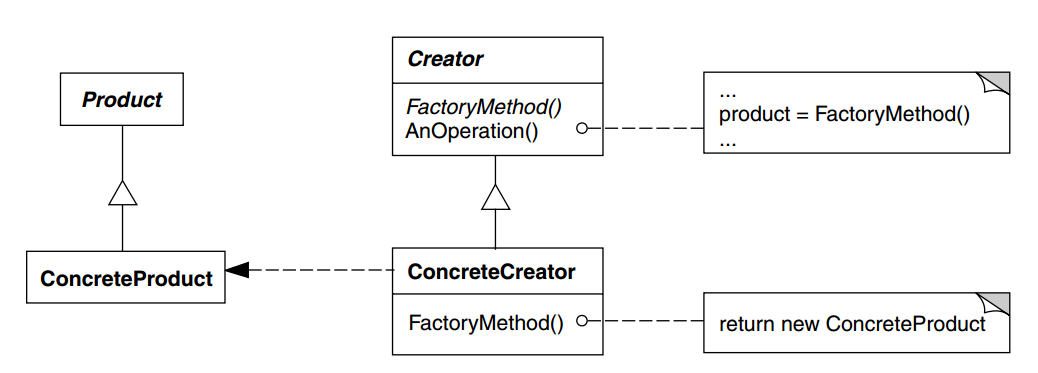
\includegraphics[scale=0.5]{5_padroes-contexto-funcional/5.1_criacionais/5.1.1_factory-method/diagram.png}
	\end{center}
\end{figure}

Exemplo Orientado a Objetos:

\begin{lstlisting}[caption={Factory Method Orientado a Objetos},label=oofactory]
    
    trait Product{
        def doStuff() : Unit
    }

    class ConcreteProduct extends Product(){

        def doStuff() : Unit = {
            
        }
    }

    abstract class Creator(){

        def someOperation() : Unit = {
            var p = createProduct()
            p.doStuff()
        }

        def createProduct() : Product
    }

    class ConcreteCreator() extends Creator{

        def createProduct() : Product = {
            return new ConcreteProduct()
        }
    }

\end{lstlisting}

Contexto Funcional:

\begin{lstlisting}[caption={Factory Method Funcional},label=fpfactory]
    
    

\end{lstlisting}

\section{Abstract Factory}

O padrão \textit{Abstract Factory} define uma família 
de objetos relacionados e uma interface para 
criá-los, sem definir sua implementação. Dessa 
forma, diferentes implementações desse 
conjunto de objetos podem ser utilizadas 
sem que as classes cliente que os utilizam 
precisem conhecê-las.\cite{gamma:1995}

O diagrama apresentado na Figura \ref{abfactory_struct} 
demonstra a estrutura desse padrão, onde a 
interface \texttt{AbstractFactory} suporta as famílias 
\texttt{ConcreteFactory1} e \texttt{ConcreteFactory2}, com cada uma 
delas definindo qual implementação das interfaces 
\texttt{AbstractProductA} e \texttt{AbstractProductB} serão 
utilizadas.

\begin{figure}[htb]
	\caption{\label{abfactory_struct}Estrutura do \textit{Abstract Factory}.}
	\begin{center}
	    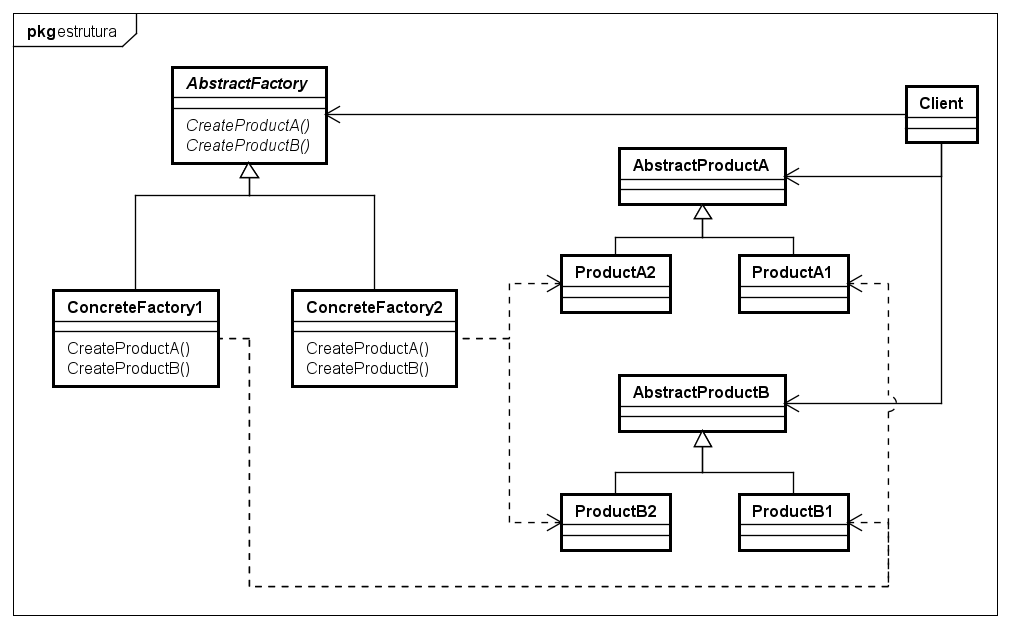
\includegraphics[scale=0.5]{5_padroes-contexto-funcional/5.1_criacionais/5.1.2_abstract-factory/abstractfactory_estrutura.png}
	\end{center}
  \caption*{Fonte: O Autor (2021)}
\end{figure}

\subsection*{Exemplo Orientado a Objetos}

Como exemplo, é apresentado um \textit{toolkit} 
que suporta tipos diferentes de interação para 
seus \textit{widgets}, como \textit{Motif} ou \textit{Presentation 
Manager} (PM). Dessa forma, para que o \textit{toolkit} 
não precise ser implementado tendo conhecimento 
de cada tipo diferente de \textit{widget}, é 
utilizado o padrão \textit{Abstract Factory} para 
definir uma família de objetos de \textit{widget} 
diferente para cada tipo de interação. 

A implementação do padrão é demonstrada no 
diagrama de classes da Figura \ref{abfactory_exemplo} 
e no Código \ref{ooabfactory}. Uma interface 
\texttt{WidgetFactory} define as operações de criação 
de todos os \textit{widgets} possíveis, enquanto 
as classes \texttt{MotifWidgetFactory} e \texttt{PMWidgetFactory} 
implementam sua criação para os tipos de 
interação suportados.

\begin{figure}[htb]
	\caption{\label{abfactory_exemplo}Exemplo de \textit{Abstract Factory}.}
	\begin{center}
	    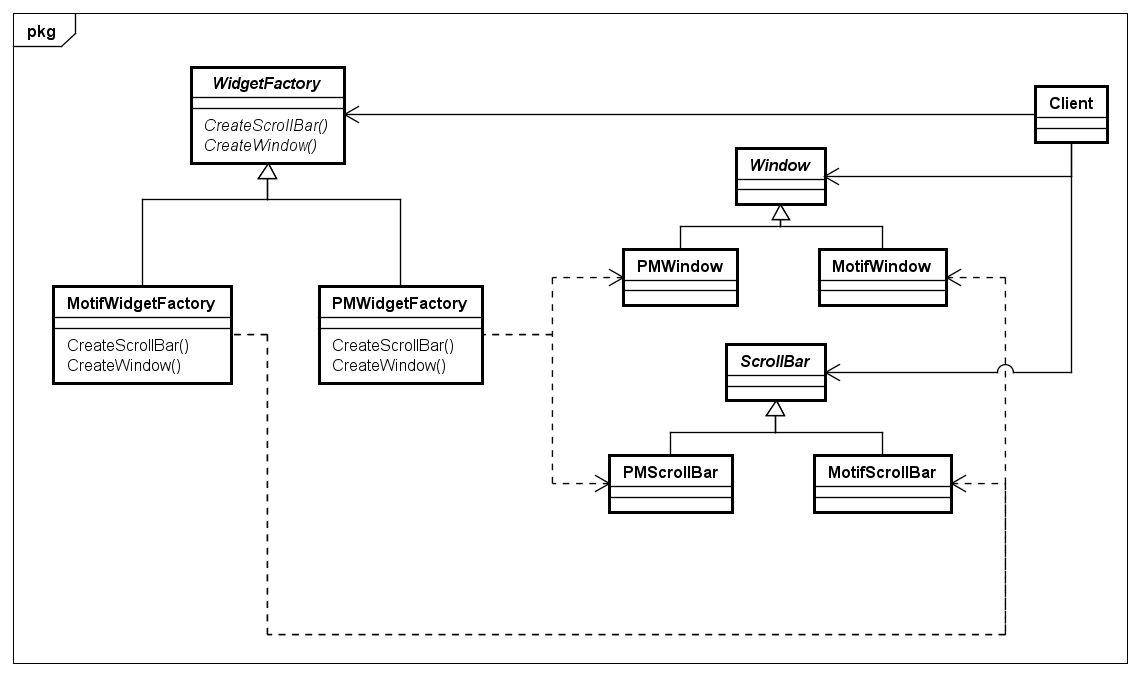
\includegraphics[scale=0.5]{5_padroes-contexto-funcional/5.1_criacionais/5.1.2_abstract-factory/abstractfactory_exemplo.png}
	\end{center}
  \caption*{Fonte: O Autor (2021)}
\end{figure}

\begin{lstlisting}[caption={\textit{Abstract Factory} Orientado a Objetos.},label=ooabfactory]
	
trait WidgetFactory {
  def CreateScrollBar() : ScrollBar
  def CreateWindow() : Window
}

trait Window 
trait ScrollBar

class MotifWidgetFactory extends WidgetFactory {
  def CreateScrollBar(): ScrollBar = new MotifScrollBar()
  def CreateWindow(): Window = new MotifWindow()
}

class PMWidgetFactory extends WidgetFactory {
  def CreateWindow(): Window = new PMWindow()
  def CreateScrollBar(): ScrollBar = new PMScrollBar()
}

class PMWindow extends Window {
  // Implementação de PMWindow
}

class MotifWindow extends Window {
  // Implementação de MotifWindow
}

class PMScrollBar extends ScrollBar {
  // Implementação de PMScrollBar
}

class MotifScrollBar extends ScrollBar {
  // Implementação de MotifScrollBar
}

\end{lstlisting}
\legend{Fonte: O Autor (2021)}


\subsection*{Contexto Funcional}

As classes e interfaces \textit{factory} podem 
ser substituídas por funções de alta ordem 
recebidas pela função cliente. 
No Código \ref{fpabfactory} são definidos, 
nas linhas 2 e 3,  
os tipos \texttt{ScrollBar} e \texttt{Window} referentes aos 
\textit{widgets} suportados pela ferramenta. 
Da mesma forma, são definidas as operações de 
criação desses \textit{widgets} para os tipos 
\texttt{PM} e \texttt{Motif}. Nas linhas 5 e 8 são definidas as 
operações para o tipo \texttt{PM}, enquanto nas linhas 
12 e 15 são definidas as para o tipo \texttt{Motif}. 

Na linha 19 é definida uma função cliente, 
que seria equivalente a uma operação da classe 
\texttt{Client} apresentada no diagrama da Figura 
\ref{abfactory_exemplo}. Ela 
recebe como parâmetro as funções para criação de 
cada \textit{widget}. Por fim, na linha 28 é 
demonstrada a chamada dessa função recebendo 
como parâmetro as funções para criar um 
\textit{scrollbar} e uma janela para o tipo 
\texttt{PM}.

\begin{lstlisting}[caption={\textit{Abstract Factory} Funcional.},label=fpabfactory]
    
type Scrollbar
type Window

def CreatePMScrollBar() : Scrollbar = {
  // Criação da scrollbar PM
}
def CreatePMWindow() : Window = {
  // Criação da janela PM
}

def CreateMotifScrollBar() : Scrollbar = {
  // Criação da scrollbar Motif
}
def CreateMotifWindow() : Window = {
  // Criação da janela Motif
}

def ClientFunction(
  scrollBarFactory : () => Scrollbar, 
  windowFactory : () => Window): Unit = {
  // ...
  val scrollbar = scrollBarFactory()
  val window = windowFactory()
  // ...
}

ClientFunction(CreatePMScrollBar, CreatePMWindow)

\end{lstlisting}
\legend{Fonte: O Autor (2021)}

No Código \ref{fpabfactory}, seria possível passar 
para a classe cliente \textit{widgets} de tipos 
misturados, já que são definidos parâmetros 
diferentes para cada função de criação. Caso 
seja desejado um exemplo mais próximo do demonstrado 
no diagrama da Figura \ref{abfactory_exemplo}, 
pode-se encapsular as funções de criação 
em uma tupla. Isso pode ser visto no Código 
\ref{fpabfactory2}, onde o tipo \texttt{WidgetFactory} 
definido na linha 2 armazena tanto uma função 
para a criação de um \textit{scrollbar} quanto a função 
para a criação de uma janela. A função 
cliente, redefinida na linha 10, agora 
recebe como parâmetro um valor do tipo 
\texttt{WidgetFactory}.

\begin{lstlisting}[caption={\textit{Abstract Factory} Funcional usando tuplas.},label=fpabfactory2]
    
type WidgetFactory = (
  () => ScrollBar, 
  () => Window
)

val PMWidgetFactory : WidgetFactory = 
  (CreatePMScrollBar, CreatePMWindow)

def ClientFunction(factory : WidgetFactory) : Unit = // ...

ClientFunction(PMWidgetFactory)

\end{lstlisting}
\legend{Fonte: O Autor (2021)}

\section{Singleton}

O padrão Singleton garante que um objeto possuirá apenas uma 
instância. Além disso, fornece um único ponto acessível 
globalmente a essa instância. Esse padrão é útil 
para implementar classes que fornecem serviços sem que seja 
necessário instanciar vários objetos idênticos em 
locais diferentes do código.

A figura \ref{singleton_struct} demonstra a implementação 
do padrão. A classe Singleton possui um método construtor 
privado e armazena no atributo estático uniqueInstance uma 
instância de Singleton. Através do método de classe 
Instance, é verificado se já existe uma instância 
armazenada no atributo uniqueInstance. Caso já exista, 
ela é retornada. Caso não, a instância única é criada 
para ser retornada nas chamadas posteriores de Instance.

\begin{figure}[htb]
	\caption{\label{singleton_struct}Estrutura do Singleton}
	\begin{center}
	    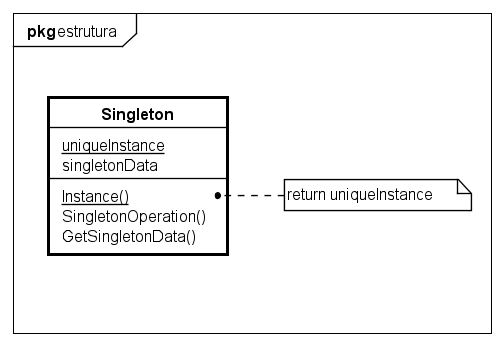
\includegraphics[scale=0.6]{5_padroes-contexto-funcional/5.1_criacionais/5.1.5_singleton/singleton_estrutura.png}
	\end{center}
\end{figure}

\subsection*{Exemplo Orientado a Objetos}

Uma classe define as operações para realizar transações com 
uma base de dados. Como a instância dela é idêntica independente 
do cliente que a utiliza, não existe a necessidade de replicar 
essas instâncias pelo código. Ela pode ser transformada em 
um Singleton, o que faz com que toda classe que deseja fazer 
uma transação na base de dados apenas solicite uma instância 
e realize as operações. A definição da classe do exemplo 
pode ser vista na figura \ref{singleton_exemplo} e no 
código \ref{oosingleton}.

\begin{figure}[htb]
	\caption{\label{singleton_exemplo}Exemplo de Singleton}
	\begin{center}
	    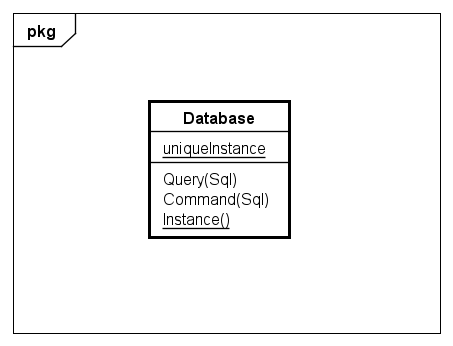
\includegraphics[scale=0.6]{5_padroes-contexto-funcional/5.1_criacionais/5.1.5_singleton/singleton_exemplo.png}
	\end{center}
\end{figure}

\begin{lstlisting}[caption={Singleton Orientação a Objetos},label=oosingleton]

class Database private(){
  def Query(sql : String) : Object = {
    //Execute query
    null
  }
  def Command(sql : String) : Unit = {
    //Execute command
  }
}

object Database {
  private var instance : Database = null

  def Instance() : Database = {
    if(instance == null){
      instance = new Database()
    }
    instance
  }
}

\end{lstlisting}

\subsection*{Contexto Funcional}

Em um contexto sem classes e objetos, 
um singleton poderia ser considerado como 
uma variável global, acessível por 
todo o programa. Essa ideia viola o conceito 
de função pura, já que uma função que acessa 
um singleton deixa de depender apenas de seus 
parâmetros. Para o caso em que o Singleton 
armazene algum estado, o conceito de imutabilidade 
também precisaria ser violado, já que o 
valor que armazena o Singleton precisaria ser 
mutável para ser alterado de dentro de uma 
função. Com isso, não existe uma implementação 
equivalente ao Singleton no contexto funcional.

% ----------------------------------------------------------
% ESTRUTURAIS
% ----------------------------------------------------------
\section{Estruturais}

% ----------------------------------------------------------
% COMPORTAMENTAIS
% ----------------------------------------------------------
\section{Comportamentais}

\subsection{Strategy}

O padrão Strategy tem como objetivo definir uma família de 
algoritmos e encapsulá-las e torná-las intercambiáveis. Dessa 
forma, uma classe que deseja utilizar algum desses algoritmos 
pode alternar entre eles dinamicamente.

\begin{figure}[htb]
	\caption{\label{fig_grafico}Estrutura do Strategy}
	\begin{center}
	    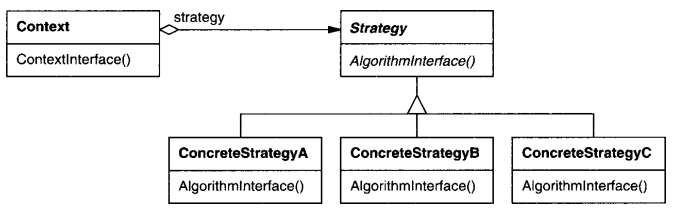
\includegraphics[scale=0.5]{5_padroes-contexto-funcional/5.3_comportamentais/5.3.9_strategy/diagram.png}
	\end{center}
\end{figure}

Exemplo Orientado a Objetos:

\begin{lstlisting}[caption={Strategy Orientação a Objetos},label=oostrategy]
    
    trait Strategy {
        def algorithmInterface() : Unit
    }

    class ConcreteStrategyA() extends Strategy {
        def algorithmInterface() : Unit = {

        }
    }

    class ConcreteStrategyB() extends Strategy {
        def algorithmInterface() : Unit = {

        }
    }

    class Context(var strategy : Strategy) {
        def setStrategy(strategy : Strategy) = this.strategy = strategy

        def contextInterface() : Unit = {
            this.strategy.algorithmInterface()
        }
    }

\end{lstlisting}

Contexto Funcional:

No contexto funcional, já que existem as funções de alta 
ordem (High-order functions), não é necessário definir 
interfaces ou classes concretas para implementar os 
algoritmos: Basta que a função desejada exista e ela 
pode ser passada por parâmetro para a operação 
ContextInterface.

\begin{lstlisting}[caption={Strategy Orientação a Objetos},label=oostrategy]
    
    def algorithmInterfaceA() : Unit = {
        
    }

    def algorithmInterfaceB() : Unit = {
        
    }

    def ContextInterface(algorithmInterface : () => Unit) : Unit = algorithmInterface()

\end{lstlisting}


% ----------------------------------------------------------
% PARTE
% ----------------------------------------------------------
\part{Resultados}
% ----------------------------------------------------------

% ---
% Apresentação dos Resultados
% ---
\chapter{Apresentação dos Resultados}
% ---

Nos capítulos anteriores, foram analisados todos 
vinte e três padrões de projeto \textit{Gang of 
Four}, com o objetivo de extrair o problema 
resolvido pelo padrão e analisar, a partir dos 
conceitos de programação funcional apresentados, 
como uma solução para o mesmo problema poderia ser 
alcançada. 

Foi possível separar as análises realizadas em 
quatro grandes grupos, com o primeiro sendo 
dividido em três subgrupos: 

\begin{alineas}
    \item Padrões resolvidos por funções de alta ordem
    \begin{alineas}
        \item Funções de alta ordem como alternativa a classes abstratas ou interfaces
        \item Valores que armazenam funções
        \item Funções que armazenam valores em closures
    \end{alineas}
    \item Padrões com soluções alternativas
    \item Padrões sem diferenças relevantes
    \item Padrões que não fazem sentido no contexto funcional
\end{alineas}

Esses grupos estão organizados na tabela 
\ref{resultados}, onde são apresentados os 
padrões pertencentes a cada grupo com a 
quantidade de padrões pertencentes ao grupo. 
Cada grupo será explicado com mais detalhes 
no decorrer do capítulo.

\begin{quadro}[htb]
    \caption{\label{resultados}Agrupamento de análises dos padrões}
    \begin{tabular}{@{}llll@{}}
        \toprule
                                  &                            & Padrões                 & Quantidade         \\ \midrule
        \multirow{14}{*}{Grupo A} & \multirow{7}{*}{A.1} & Factory Method          & \multirow{7}{*}{7} \\
                                  &                            & Builder                 &                    \\
                                  &                            & Adapter                 &                    \\
                                  &                            & Bridge                  &                    \\
                                  &                            & Proxy                   &                    \\
                                  &                            & Strategy                &                    \\
                                  &                            & Template Method         &                    \\ \cmidrule(r){2-4}
                                  & \multirow{3}{*}{A.2} & Abstract Factory        & \multirow{3}{*}{3} \\
                                  &                            & Command                 &                    \\
                                  &                            & State                   &                    \\ \cmidrule(r){2-4}
                                  & \multirow{4}{*}{A.3} & Composite               & \multirow{4}{*}{4} \\
                                  &                            & Decorator               &                    \\
                                  &                            & Chain of Responsibility &                    \\
                                  &                            & Interpreter             &                    \\ \cmidrule(r){1-4}
        \multicolumn{2}{l}{\multirow{3}{*}{Grupo B}}           & Iterator                & \multirow{3}{*}{3} \\
        \multicolumn{2}{l}{}                                   & Observer                &                    \\
        \multicolumn{2}{l}{}                                   & Visitor                 &                    \\ \cmidrule(r){1-4}
        \multicolumn{2}{l}{\multirow{3}{*}{Grupo C}}           & Façade                  & \multirow{3}{*}{3} \\
        \multicolumn{2}{l}{}                                   & Flyweight               &                    \\
        \multicolumn{2}{l}{}                                   & Mediator                &                    \\ \cmidrule(r){1-4}
        \multicolumn{2}{l}{\multirow{3}{*}{Grupo D}}           & Prototype               & \multirow{3}{*}{3} \\ 
        \multicolumn{2}{l}{}                                   & Singleton               &                    \\
        \multicolumn{2}{l}{}                                   & Memento                 &                    \\ \cmidrule(r){1-4} %\cmidrule(l){4-4} 
    \end{tabular}
\end{quadro}

\section{Padrões resolvidos por funções de alta ordem}

Entre as soluções vistas, a que é aplicada na 
maior parte dos padrões é o uso de funções de alta 
ordem como alternativa a interfaces ou classes. 
Um total de catorze dos vinte e três padrões 
se encaixa nessa categoria. Por isso, ainda foi 
possível dividir esses padrões em três  
subcategorias quanto a como as funções de alta 
ordem foram aplicadas. Alguns padrões acabam se 
encaixando em mais de uma delas, mas para 
evitar repetições e para simplificar o agrupamento, 
cada padrão será explicado no grupo mais próximo 
da solução proposta. 

% Factory Method, Builder, Adapter, Bridge, 
% Proxy, Strategy, Template Method
\subsection{Funções de alta ordem como alternativa a 
            classes abstratas ou interfaces}

Como foi visto no mapeamento de conceitos orientados 
a objeto para conceitos de programação funcional, 
funções de alta ordem podem servir como alternativas 
para o uso de interfaces. Alguns dos padrões analisados 
baseiam-se no uso de interfaces para definir a assinatura 
de funções que a classe cliente deve receber. De forma 
equivalente, é possível que uma função cliente recebe, 
por parâmetro, uma função com a assinatura equivalente 
à da interface. Essa é a abordagem utilizada com os 
padrões Builder, Adapter, Bridge, Proxy e Strategy. 

De forma semelhante, as funções de alta ordem são 
alternativas ainda mais interessantes ao uso de 
classes abstratas, como é o caso dos padrões 
Factory Method e Template Method. Ambos baseiam-se 
em definir uma operação abstrata que deve ser 
implementada por uma subclasse. Uma alternativa 
a essa implementação é fazer com que as funções 
que dependam dessa operação abstrata a recebam 
por parâmetro.

% Abstract Factory, Command, State
\subsection{Valores que armazenam funções}

Os padrões Abstract Factory, Command e 
State também baseiam-se em passar funções de 
alta ordem como parâmetro para funções clientes. 
Porém, para esses três padrões existe uma quantidade 
maior de funções que o cliente deve receber. Além 
disso, pode ser mais interessante que as implementações 
dessas funções sejam dependentes entre si, ou seja, 
todas as funções de um Strategy pertençam a uma mesma 
estratégia, todas as funções do Abstract Factory criem 
o mesmo tipo de valor e a função de desfazer do 
Command esteja relacionada à função principal executada. 
Agrupar essas funções em um mesmo valor pode 
contribuir para retirar das funções clientes a 
responsabilidade de garantir que elas possuam 
essa equivalência.

% Composite, Decorator, Chain of Responsibility, Interpreter
\subsection{Funções que armazenam valores em closures}

Algumas implementações basearam-se em definir funções 
que retornam novas funções. Isso é necessário para 
que seja possível configurar as funções retornadas 
com valores recebidos por parâmetro pelas funções 
que as criam. Esse é o comportamento definido pelas 
closures, onde uma determinada função armazena 
um valor do escopo da função que a retornou. 

O padrão Composite define funções para gerar os 
elementos nós e os elementos folha. Dessa forma, 
a partir de uma única função, vários elementos 
folha e nó configurados com valores diferentes 
podem ser gerados.

De forma semelhante, o padrão Decorator define 
funções que podem receber como parâmetro valores 
variados enquanto retorna uma nova função com 
a mesma assinatura da função decorada. 

O padrão Chain of Responsibility aproveita a mesma 
ideia para gerar as funções da cadeia. O tópico e 
a próxima função da cadeia são passadas por parâmetro 
previamente, armazenadas na closure e reaproveitadas 
na função retornada. 

Por fim, o padrão Interpreter apresenta um comportamento 
semelhante ao Composite, definindo funções que retornam 
os elementos terminais e não terminais, permitindo 
inclusive definir funções mais genéricas que recebem 
a função que aplica a regra da gramática por parâmetro.

% Iterator, Observer, Visitor
\section{Padrões com soluções alternativas}

Os padrões Iterator, Observer e Visitor possuem 
implementações alternativas que não necessariamente 
seguem à risca a ideia do padrão. No caso do Iterator, 
existe a diferença entre o gerencimaneto por parte 
do cliente e por parte da coleção entre as 
alternativas orientada a objetos e funcional. No 
caso do Observer, o conceito no qual ele se 
baseia - programação reativa - é levado em 
consideração ao substituí-lo pela programação 
reativa funcional. Já o Visitor, apesar de também 
aproveitar-se de funções de alta ordem, na verdade 
é resolvido pelo recurso \textit{pattern matching}, 
que não é um conceito exclusivamente funcional, 
porém costuma ser implementado em linguagens 
funcionais. Nesse caso, o padrão não foi 
resolvido por programação funcional em si, 
mas sim por uma alternativa próxima. 

% Façade, Flyweight, Mediator
\section{Padrões sem diferenças relevantes}

Alguns dos padrões analisados possuem 
uma implementação muito semelhante ou 
equivalente entre os contextos orientados 
a objeto e funcionais, como se a solução 
proposta pelo padrão estivesse apenas 
sendo reutilizada por si só, sem 
recursos adicionais oriundos da programação 
funcional que contribuem para a 
resolução do problema. 

Da mesma forma que o padrão Façade orientado 
a objetos baseia-se no acesso entre as classes, 
a implementação funcional baseia-se no acesso 
entre módulos. Como ambas as ideias são 
análogas, a implementação do padrão na verdade 
não possui mudanças significativas. 

Da mesma forma, o padrão Flyweight, tanto no 
contexto orientado a objetos quanto no funcional, 
é implementado através de memoização. Já o Mediator 
baseia-se em possuir uma função (ou classe) que 
gerencia as dependências entre valores (ou objetos). 
No caso desses dois padrões, ambos possuem 
pequenas diferenças como consequência de suas 
implementações - por exemplo, não existem os dois 
tipos de Flyweight intrínseco ou extrínseco 
graças à imutabilidade e há a necessidade do 
cliente gerenciar a mudança de estado dos 
\textit{colleagues} no Mediator -, mas a ideia 
por trás da implementação de ambos é análoga 
à versão orientada a objetos.

% Prototype (imutabilidade), Singleton (funções puras), 
% Memento (imutabilidade)
\section{Padrões que não fazem sentido no contexto funcional}

Para alguns padrões, o problema proposto deixa 
de existir graças aos conceitos já implementados 
em linguagens funcionais. No caso dos padrões 
analisados neste trabalho, encaixam-se nessa 
categoria o Singleton, o Prototype e o Memento. 

Como a intenção do padrão Singleton pode 
ser entendida como a definição de uma variável 
global, sua implementação no contexto funcional 
viola o conceito de funções puras e imutabilidade - 
para o caso em que o Singleton armazena algum 
estado compartilhado. Portanto, tentar 
implementá-lo não faz sentido. 

Para o caso do Prototype, como visto anteriormente, 
o uso de estruturas de dados imutáveis trazem um 
gerenciamento mais simples de memória. Não existe 
preocupação quanto a uma referência compartilhada 
para um mesmo valor, já que seu estado não pode ser 
modificado. Dessa forma, não há a necessidade de 
definir uma implementação que compartilhe dados.

Por fim, o padrão Memento, também graças à 
imutabilidade, não precisaria se preocupar quanto 
a expor o estado interno de um valor. Assim, é 
possível gerar \textit{snapshots} apenas copiando 
valores anteriores, sem preocupações adicionais. 


% ---
% Conclusão
% ---
\chapter{Conclusão}
% ---

\lipsum[31-33]


% ----------------------------------------------------------
% Finaliza a parte no bookmark do PDF
% para que se inicie o bookmark na raiz
% e adiciona espaço de parte no Sumário
% ----------------------------------------------------------
\phantompart


% ----------------------------------------------------------
% ELEMENTOS PÓS-TEXTUAIS
% ----------------------------------------------------------
\postextual
% ----------------------------------------------------------

% ----------------------------------------------------------
% Referências bibliográficas
% ----------------------------------------------------------
\bibliography{abntex2-modelo-references}





%---------------------------------------------------------------------
% INDICE REMISSIVO
%---------------------------------------------------------------------
\phantompart
\printindex
%---------------------------------------------------------------------

\end{document}
